%==============================================================================
%== template for LATEX poster =================================================
%==============================================================================
%
%--A0 beamer slide-------------------------------------------------------------
\documentclass[final]{beamer}
\usepackage[orientation=portrait,size=a0,
            scale=1.25         % font scale factor
           ]{beamerposter}

\geometry{
  hmargin=2.5cm, % little modification of margins
}

%
\usepackage[utf8]{inputenc}
% diminuir o tamanho da legenda das imagens
\usepackage[font=small,labelfont=bf]{caption}

% pacotes para fluxograma
\usepackage{tikz}
\usetikzlibrary{shapes,arrows}

\renewcommand{\figurename}{Figura}

\linespread{1.15}
%
%==The poster style============================================================
\usetheme{sharelatex}

%==Title, date and authors of the poster=======================================
\title
[24$^{o}$ Simpósio Internacional de Iniciação Científica da USP] % Conference
{ % Poster title
The Fate of Man-made Radionuclides in a Semi-Enclosed Basin
}

\author{ Silva, Danilo A.\inst{1}, Castro Filho, Belmiro M.\inst{2} $\&$ Dottori, Marcelo\inst{3}
}
\institute[Instituto Oceanográfico - Universidade de São Paulo]
{
Instituto Oceanográfico da Universidade de São Paulo (IOUSP)\\ [0.2ex]
\inst{1} danilo2.silva@usp.br; \inst{2} bmcastro@usp.br; \inst{3} mdottori@usp.br
}
\date{\today}



\begin{document}

\begin{frame}
%==============================================================================
\begin{multicols}{2}
%==============================================================================
%==The poster content==========================================================
%==============================================================================

\section{Introduction}

In a global scale, water reservoirs are used to dump material from power plants and
industries, where the biggest impact occur in areas with low circulation and water
exchange with open ocean. In the context of nuclear power plants, 96$\%$ are installed
closest to water bodies, using this waters in the cooling system. In Brazil, there is
two nuclear power plants in operation, located in the Almirante Alvaro Alberto 
Central Nuclear (AAACN), that captures and discharge water in the Ilha Grande Bay
(Figure~\ref{fig:areaestudo}), region with great touristic and social ambiental importance.

Understand the circulation patterns in this region is important to avaliate how the nuclear
material will disperse supporting the stakeholders, in the case of a nuclear leakage, such
as occurred in Fukushima, in 2011.

This study aims to investigate how wind and tide force the dispersion of these radioactive material in the
estuary system and where they will affect with greater impact.

\vspace{.1in}
\begin{figure}
\centering
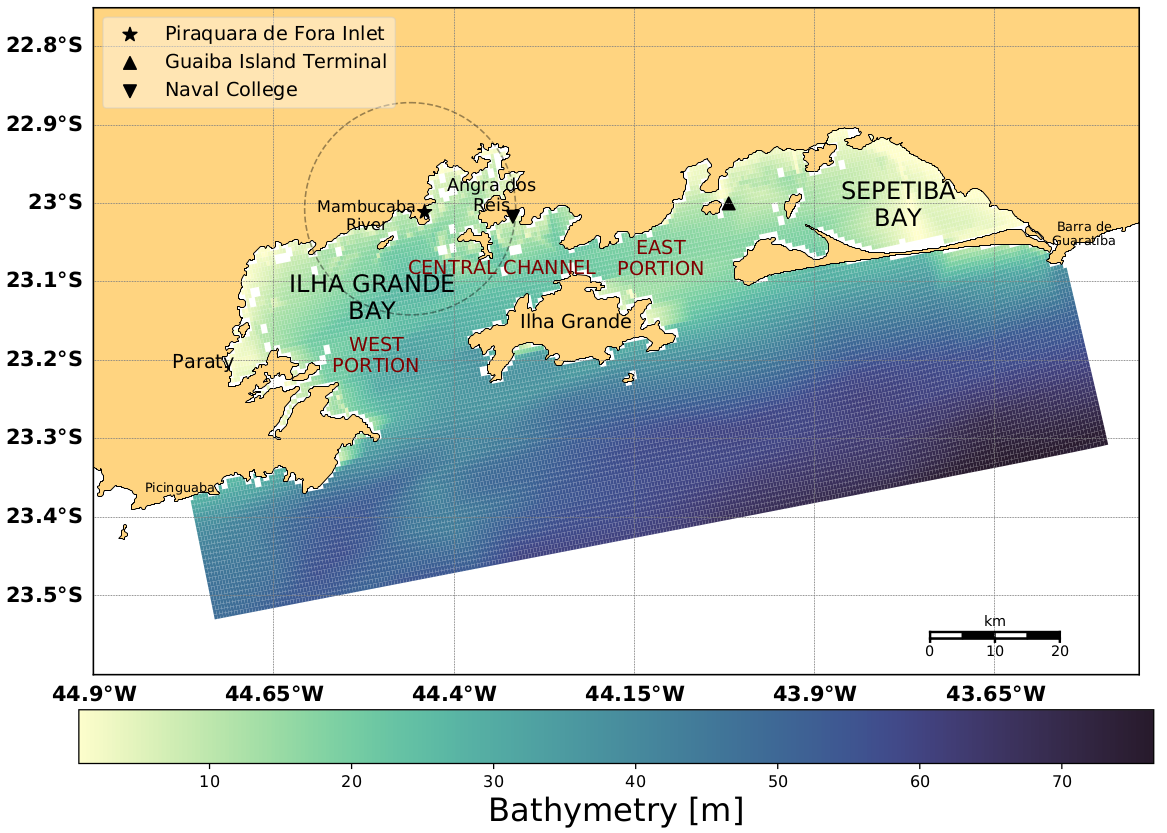
\includegraphics[width=0.8\columnwidth]{/home/tparente/danilo/mestrado/github/congressos/iwmo2018/figs/fig1.png}
\vspace{.1in}
\caption{The Ilha Grande and Sepetiba Bay domain used for ECOM model runs, showing bathymetry in meters. Several sites that are discussed in the paper are shown.}
\label{fig:areaestudo}
\end{figure}
% \vskip1ex
\vspace{-.5in}
% ===================================================================================================================
\section{Methods}

% Para determinar como o vento e a maré,
% principais forçantes, atuam na região, utilizou-
% se o \textit{Stevens Estuarine and Coastal
% Ocean Model}, ou sECOM.
% O modelo possui diversos módulos,
% onde ó módulo hidrodinâmico foi o utilizado
% para modelar a influência de cada variável
% na circulação da região.

\vskip1ex
\begin{figure}
\centering
\includegraphics[width=0.69\columnwidth]{/home/tparente/danilo/mestrado/github/congressos/iwmo2018/figs/diagramaTGFINAL1.png}
\vspace{.2in}
\caption{Scheme of the method applied in this work, where the read boxes represent input data, black boxes the modules from
ECOM and the blue boxes represent the experiments performed in this work.}
\label{fig:metodologia}
\end{figure}
\vskip1ex

\vspace{-.7in}
% ===================================================================================================================

\section{Results and Discussions}

\subsection{Wind v. Tide: Surface Circulation}

Was observed an intense eastward current in central channel in the Experiment I, with northeasterly winds, 
associated to South America Subtropical High, reaching velocities closest to 0.25 $m.s^{-1}$, while in the Experiment II, with winds associated to Frontal Systems passage, such current reach a maximum of 0.23 $m.s^{-1}$, with a westward direction. The difference between those two experiments, considering the same wind's intensity, may be cause by the open area available for southwesterly wind. Finally, in the Experimet III, only with tides from TPXO 7.2, present the highest velocities, concentrated in the eastern region of modelled domain, with maximum of 0.6 $m.s^{-1}$ during flood spring tide.

% \vskip.5ex
\begin{figure}
\centering
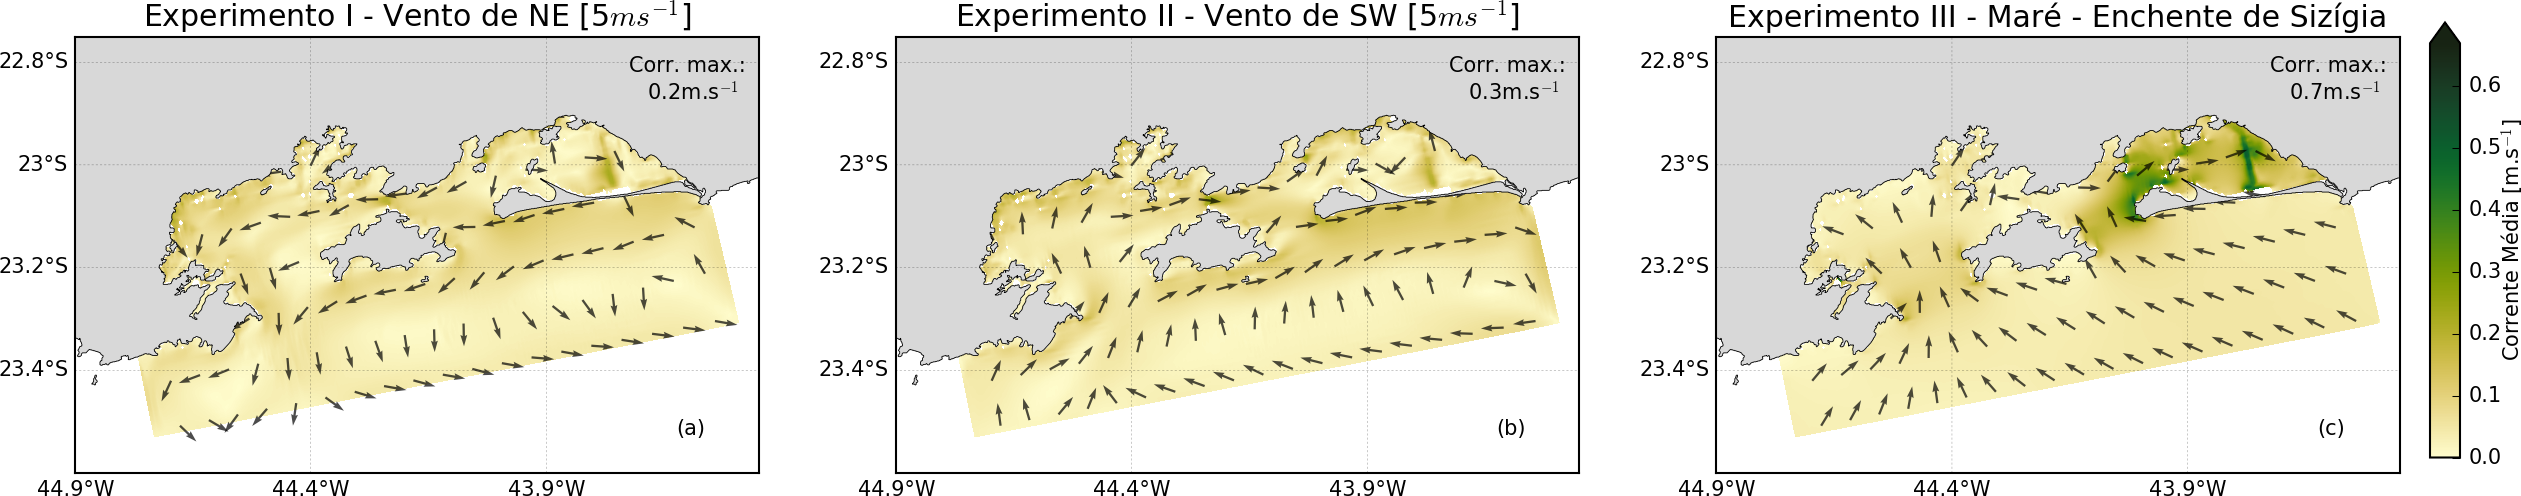
\includegraphics[width=1.\columnwidth]{/home/tparente/danilo/mestrado/github/congressos/iwmo2018/figs/figura1.png}
\caption{Corrente média nos cenários 1,2 e 3. Os painéis (a) e (b) representam o último instante modelado e (c), o instante da segunda maré enchente de sizígia do período modelado.}
\label{fig:cenariosCirc}
\end{figure}
\vspace{-1ex}

In Experiments V and VI, all variables are used (tide, wind and fluvial discharge), with
variable winds based on typical values, like in the Experiments I and II, respectively. 
In these scenarios, we identify that southwesterly winds induce the strongest surface
currents, with mean values of 0.43 $m.s^{-1}$ (Figure~\ref{fig:cenariosDispersao}.a 
and~\ref{fig:cenariosDispersao}.b). Despite the influence of the tide in more intense currents, 
the surface current direction will be controlled by the direction of the wind 
(Figure~\ref{fig:cenariosDispersao}.c and~\ref{fig:cenariosDispersao}.d), 
consequenty, controlling the direction of the radioactive material direction.
The tide, in this case, will be the main mechanism acting on advection of radioactive
material.

\begin{figure}
\centering
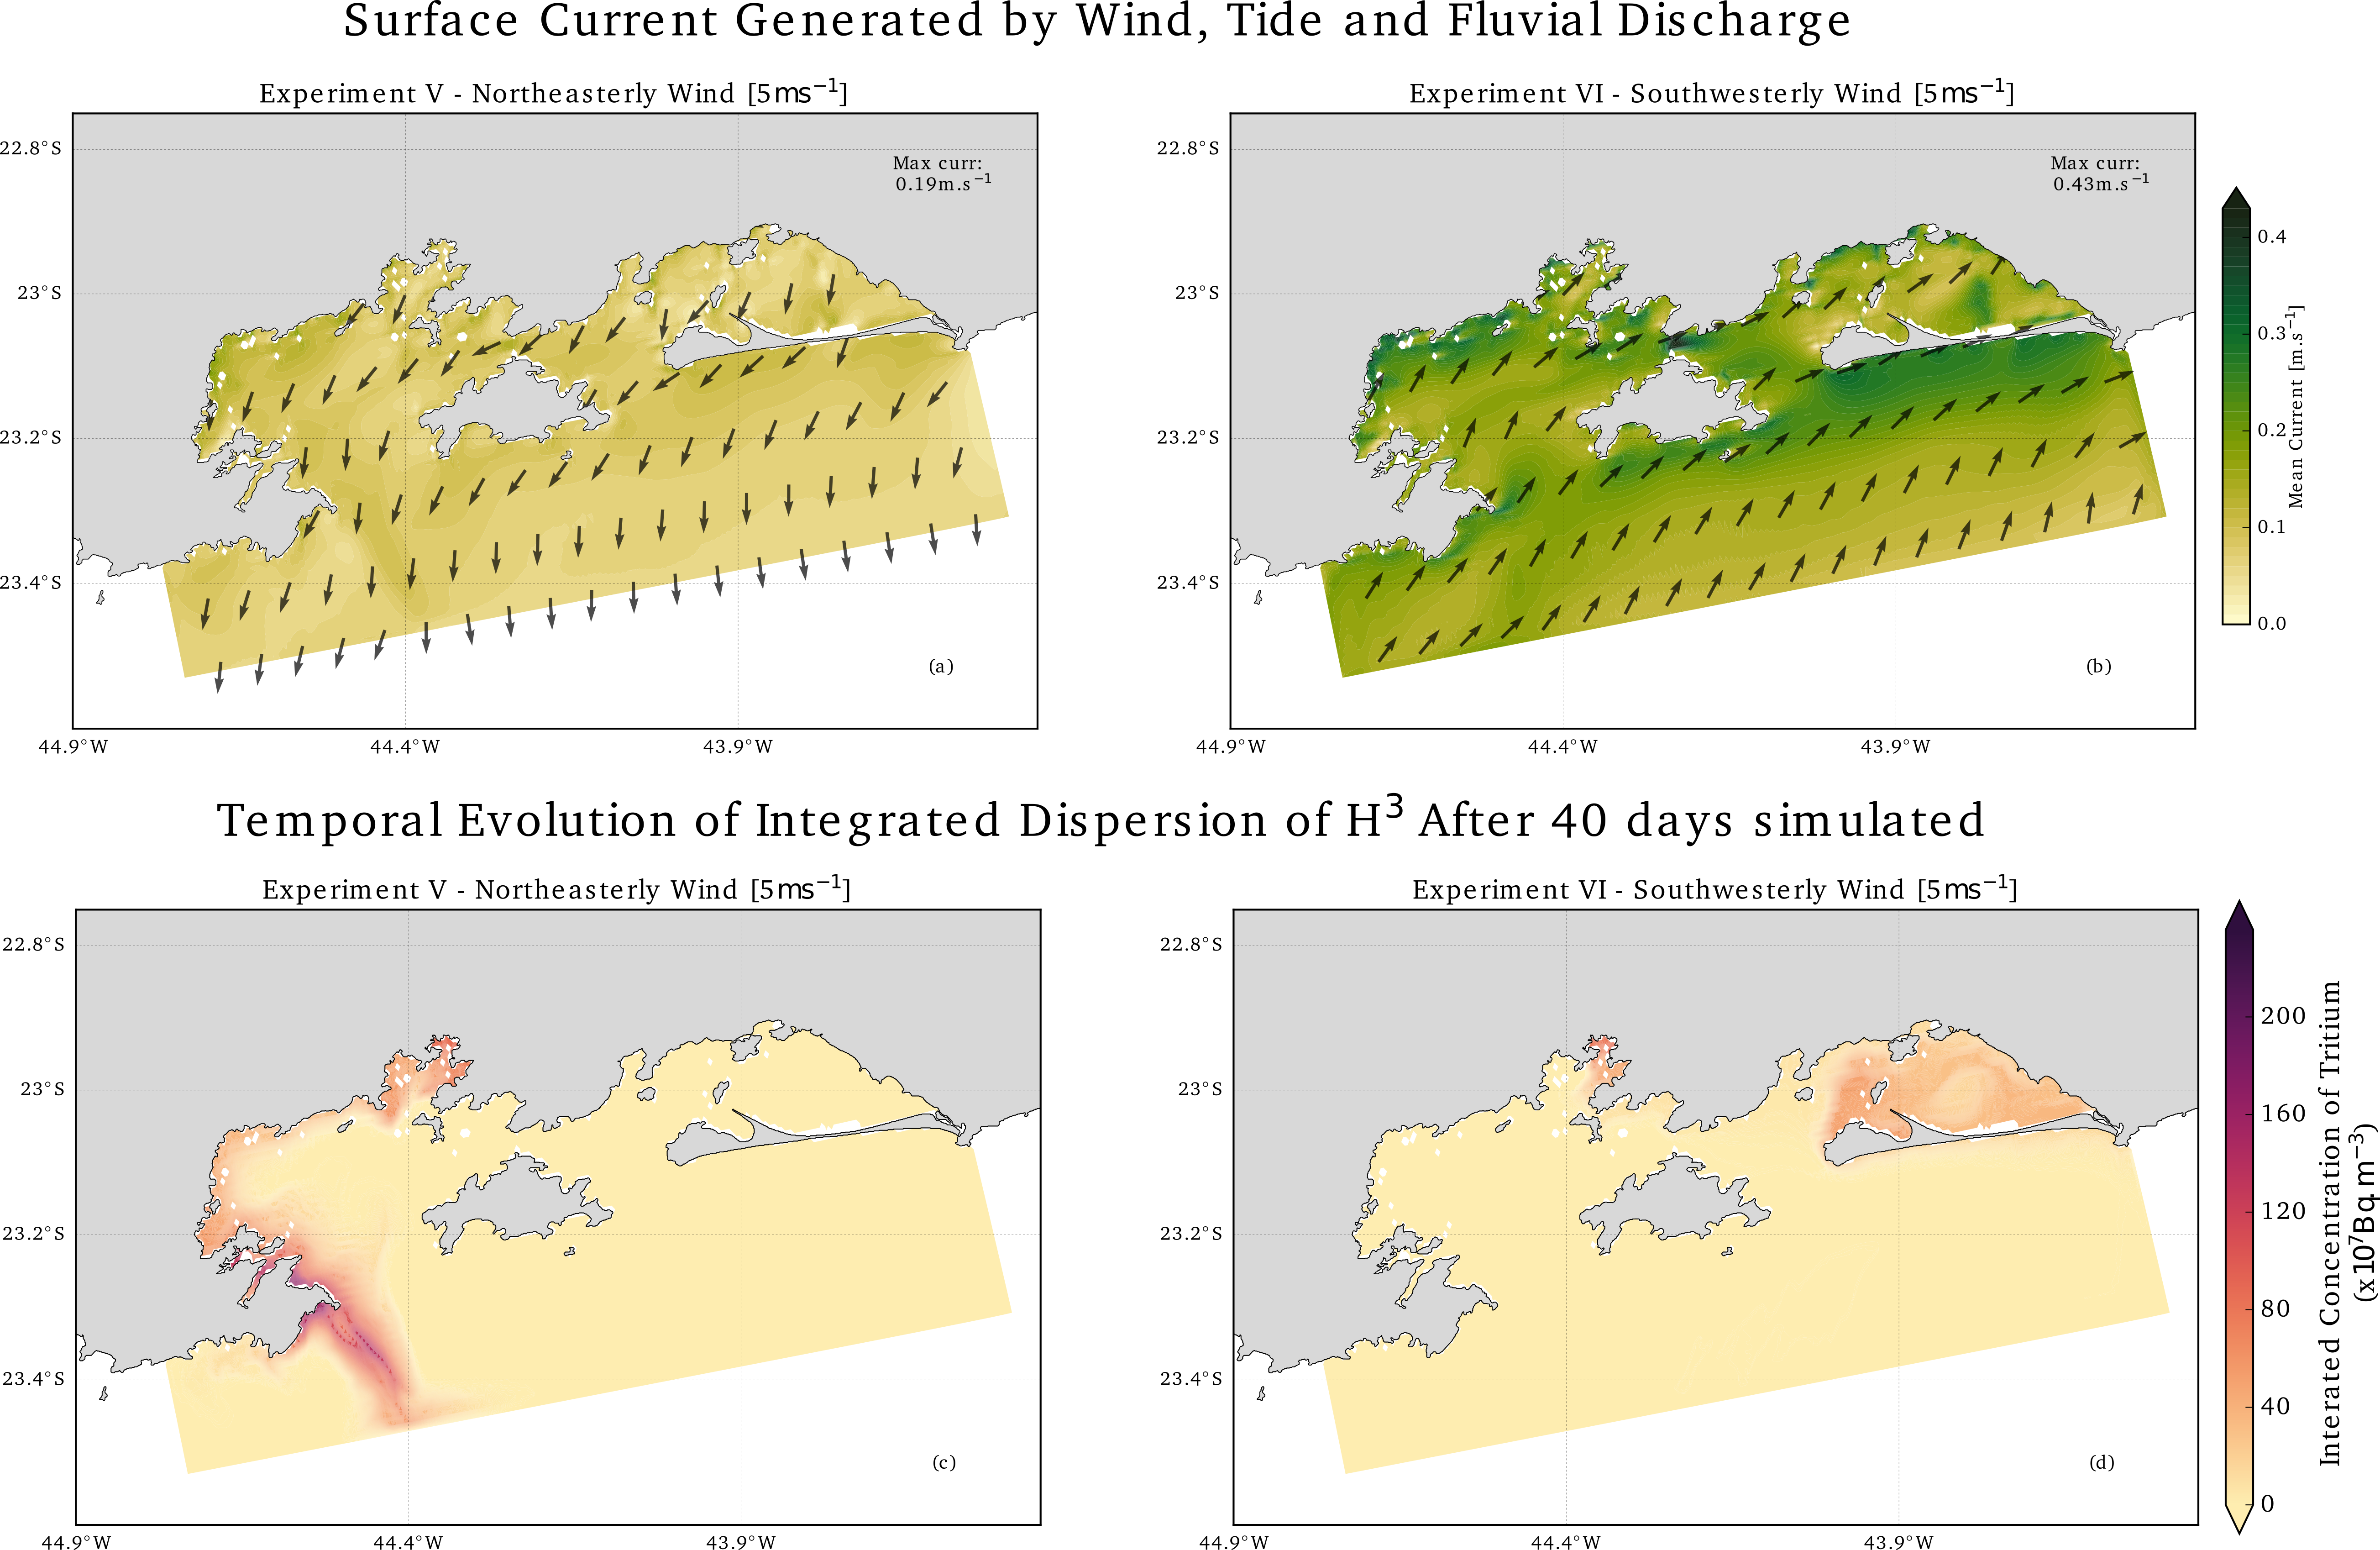
\includegraphics[width=0.99\columnwidth]{/home/tparente/danilo/mestrado/github/congressos/iwmo2018/figs/fig2_combined.png}
\caption{Mean surface current on the upper panels and integrated dispersion on the inferior panels.}
\label{fig:cenariosDispersao}
\end{figure}

\subsection{Dispersion in a Scenario Under Nearest to Real Conditions}


%Quanto ao cenário 7 (Figura~\ref{fig:evolucaopluma}), observou-se que a evolução da pluma ocorre,
%preferencialmente, para leste do domínio, conforme no cenário 5, onde parte dela
%permanece por mais de 30 dias na Baía da Ribeira e outra parte é transportadapara regiões de
%correntes mais intensas, sendo rapidamente diluídas. Baseando-se nos cenários 5,6 e 7,
%estima-se que levaria mais de 60 dias para que grande parte do material fosse diluído na
%região, o que poderia acarretar em sérios problemas para a biota local, onde o material nuclear
%seria bio incorporado nos organismos e no sedimento, passando a fazer parte da cadeia alimentar.

%O tempo de permanência é melhor apresentado através da . Notamos
%que, de aproximadamente 150 horas a 500 horas, há uma grande concentração de material nuclear
%na Baía da Ribeira, região de descarte da Central Nuclear. A pluma alcança a região de
%Angra dos Reis a partir das 150 horas simuladas, permanecendo nessa região com uma
%concentração aproximadamente constante até o final da simulação.

In condition closest to real, we identify that the radioactive material will evolve 
to the east, reaching areas with more intense currents and, consequently, with
greater mixing of the pollutant. Locally, the material will stay in the northwest 
of Angra dos Reis, region where [3] identified the higher concentrations
in the surface sediment, corroborating with the informations obtained through the
hydrodynamics modelling.

\vskip-.2ex
\begin{figure}
\centering
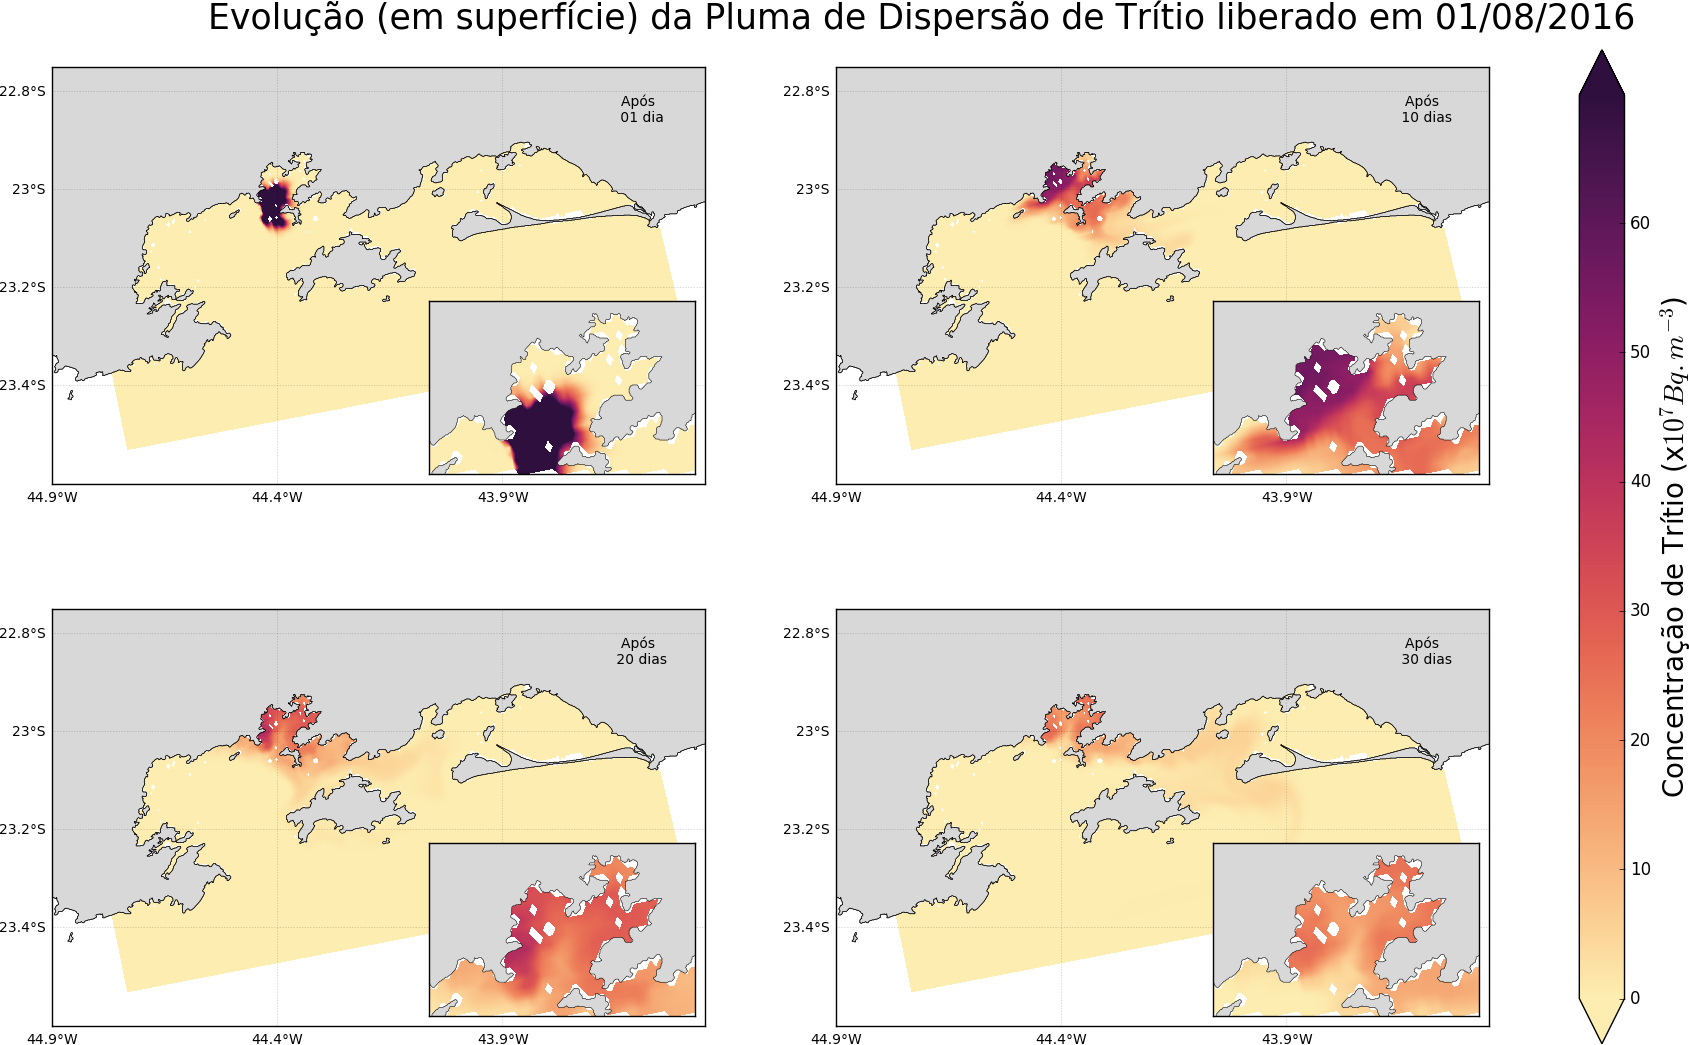
\includegraphics[width=0.9\columnwidth]{/home/tparente/danilo/mestrado/github/congressos/iwmo2018/figs/figura3_superficie.png}
\caption{Temporal evolution of the radioactive material under spatial and temporal wind variations.}
\label{fig:evolucaopluma}
\end{figure}
% \vskip2ex

% ===================================================================================================================
\vspace{-.5in}
\section{Conclusions}

\begin{itemize}
	\item Wind control direction;
	\item Tide control the mixing;
	\item In closest to real condition, the plume evolves to regions with more intense currents and
	\item The most impacted region is Angra dos Reis, followed by Central Channel and 
	Mambucada River and, finally, the East Portion is the main area of mixing.
\end{itemize}
%Conclui-se que, em caso de vazamento nuclear na CNAAA, a presença do material
%radioativo nas águas da região de estudo seria de, no mínimo, 60 dias, até uma redução a
%níveis de concentração inferiores ao previsto na resolução no283 do CONAMA.
%Além disso, as regiões de maior impacto seriam: Baía da Ribeira, ponto de descarte da
%água e, dependendo do regime de ventos no instante do vazamento, a pluma poderá
%alcançar regiões a oeste, como Paraty e Mambucaba, ou a leste, como Angra dos Reis,
%Baía de Sepetiba e Marambaia.
%Destaca-se que a pluma será melhor diluída ao atingir regiões a leste do
%domínio estudado, onde a maré gera correntes mais intensas.

\end{multicols}

%==============================================================================
\end{frame}
\end{document}
